% Foliensatz: "AFu-Kurs nach DJ4UF" von DK0TU, Amateurfunkgruppe der TU Berlin
% Lizenz: CC BY-NC-SA 3.0 de (http://creativecommons.org/licenses/by-nc-sa/3.0/de/)
% Autoren: Felix Baum DB4UM <baum@campus.tu-berlin.de>
% Korrekturen: Lars Weiler <dc4lw@darc.de>, Sebastian Lange <dl7bst@dk0tu.de>

% TODO Quellenangaben sind ein Wildwuchs -> vereinheitlichen
% TODO Widerholungspart eindeutiger markieren und schnell abarbeiten

\documentclass[aspectratio=169]{beamer}

\usepackage[ngerman]{babel} % deutsche Worttrennung etc.
\usepackage[utf8]{inputenc} % UTF8 Text

\usepackage[super, comma, numbers, square, sort]{natbib}

\usepackage{hyperref}       % Hyperref Package für bessere Referenzen (todo)
\hypersetup{
	colorlinks=false,       %   false: boxed links; true: colored links
    %linkcolor=white,       %   color of internal links (change box color with linkbordercolor)
    citecolor=red,          %   color of links to bibliography
    filecolor=white,        %   color of file links
    urlcolor=blue           %   color of external links
}

\usepackage{multirow}
\usepackage{wasysym}  % Math Symbols like \permil
%\usepackage{colortbl}
%\usepackage{subscript}
%\usepackage{caption}
%\usepackage{setspace}
%\usepackage{xcolor}        % benutze CodeListe

% Footnote
%\usepackage{hanging}
%
%\setbeamertemplate{footnote}{%
%  \hangpara{2em}{1}%
%  \makebox[2em][l]{\insertfootnotemark}\footnotesize\insertfootnotetext\par%
%}


%\usepackage{pgf}
%\usepackage{tikz}
%\usetikzlibrary{arrows,automata}
%\usetikzlibrary{positioning}
%
%\tikzset{
%    state/.style={
%           rectangle,
%           rounded corners,
%           draw=black, very thick,
%           minimum height=2em,
%           minimum width=2pt,
%           inner sep=2pt,
%           text centered,
%           },
%}

%\usepackage{listings}
%\lstset{basicstyle=\small, numberstyle=\tiny, extendedchars=true, numbers=left, numbersep=5pt}
%\lstset{showtabs=false, showspaces=false, showstringspaces=false}
%%\lstset{backgroundcolor=\color{white!75!lightgray}, , frame=single}
%%\lstset{backgroundcolor=\color{white}}
%%\lstset{backgroundcolor=none}
%\lstset{keywordstyle=\color{blue!50!gray},  identifierstyle=\color{black}}
%\lstset{commentstyle=\color{green!50!gray}, stringstyle=\color{red!50!gray}}
%\lstset{language=C, fontadjust=true, tabsize=2, breaklines=true}
%\lstset{backgroundcolor=\color{white!75!lightgray}, caption=\lstname, frame=single}
%\lstset{emphstyle=\color{black}\fbox}
%
%% Keine "Listing:"-Caption
%\captionsetup{labelformat=empty,labelsep=none}
%
%% für mathematische Umgebungen
%\usepackage{amsmath,amsfonts,amssymb}
%
%\lstdefinestyle{Bash}{
%language=Bash,
%frame=single,
%rulecolor=\color{black},
%backgroundcolor=\color{gray!50},
%keywordstyle=\color{black},
%identifierstyle=,
%commentstyle=\color{black},
%stringstyle=\color{magenta!65!white},
%showstringspaces=false,
%basicstyle=\footnotesize\ttfamily\color{black},
%numbers=none,
%breaklines=true,
%captionpos=b
%}

%\usepackage{listings}
%
%\lstdefinestyle{basic}{
%    captionpos=t,%
%    basicstyle=\footnotesize\ttfamily,%
%    numberstyle=\tiny,%
%    numbers=left,%
%    stepnumber=1,%
%    frame=single,%
%    showspaces=false,%
%    showstringspaces=false,%
%    showtabs=false,%
%    %
%    keywordstyle=\color{blue},%
%    identifierstyle=,%
%    commentstyle=\color{gray},%
%    stringstyle=\color{magenta}%
%}



% fließende Boxen haben keinen Abstand
%\fboxsep0mm

% inkludiere Creative Commons Helper
%%%%%%%%%%%%%%%%%%%%%%%%%%%%%%%%%%%%%%%%%%%%%%%%%%%%%%%%%%%%%%%%
%% ccBeamer 0.1, 2007-07-02                                   %%
%% Written by Sebastian Pipping <webmaster@hartwork.org>      %%
%% ---------------------------------------------------------- %%
%% Licensed under Creative Commons Attribution-ShareAlike 3.0 %%
%% http://creativecommons.org/licenses/by-sa/3.0/             %%
%%%%%%%%%%%%%%%%%%%%%%%%%%%%%%%%%%%%%%%%%%%%%%%%%%%%%%%%%%%%%%%%


%% Images
\newcommand{\CcImageBy}[1]{%
	
\includegraphics[scale=#1]{texdata/creative_commons/cc_by_30.pdf}%
}
\newcommand{\CcImageCc}[1]{%
	
\includegraphics[scale=#1]{texdata/creative_commons/cc_cc_30.pdf}%
}
\newcommand{\CcImageDevNations}[1]{%
	
\includegraphics[scale=#1]{texdata/creative_commons/cc_dev_nations_30.pdf}%
}
\newcommand{\CcImageNc}[1]{%
	
\includegraphics[scale=#1]{texdata/creative_commons/cc_nc_30.pdf}%
}
\newcommand{\CcImageNd}[1]{%
	
\includegraphics[scale=#1]{texdata/creative_commons/cc_nd_30.pdf}%
}
\newcommand{\CcImagePd}[1]{%
	
\includegraphics[scale=#1]{texdata/creative_commons/cc_pd_30.pdf}%
}
\newcommand{\CcImageSa}[1]{%
	
\includegraphics[scale=#1]{texdata/creative_commons/cc_sa_30.pdf}%
}
\newcommand{\CcImageSampling}[1]{%
	
\includegraphics[scale=#1]{texdata/creative_commons/cc_sampling_30.pdf}%
}
\newcommand{\CcImageSamplingPlus}[1]{%
	
\includegraphics[scale=#1]{texdata/creative_commons/cc_sampling_plus_30.pdf}%
}


%% Groups
\newcommand{\CcGroupBy}[2]{% zoom, gap
	\CcImageCc{#1}\hspace*{#2}\CcImageBy{#1}%
}
\newcommand{\CcGroupByNc}[2]{% zoom, gap
	\CcImageCc{#1}\hspace*{#2}\CcImageBy{#1}\hspace*{#2}\CcImageNc{#1}%
}
\newcommand{\CcGroupByNcNd}[2]{% zoom, gap
	\CcImageCc{#1}\hspace*{#2}\CcImageBy{#1}\hspace*{#2}\CcImageNc{#1}\hspace*{#2}\CcImageNd{#1}%
}
\newcommand{\CcGroupByNcSa}[2]{% zoom, gap
	\CcImageCc{#1}\hspace*{#2}\CcImageBy{#1}\hspace*{#2}\CcImageNc{#1}\hspace*{#2}\CcImageSa{#1}%
}
\newcommand{\CcGroupByNd}[2]{% zoom, gap
	\CcImageCc{#1}\hspace*{#2}\CcImageBy{#1}\hspace*{#2}\CcImageNd{#1}%
}
\newcommand{\CcGroupBySa}[2]{% zoom, gap
	\CcImageCc{#1}\hspace*{#2}\CcImageBy{#1}\hspace*{#2}\CcImageSa{#1}%
}
\newcommand{\CcGroupDevNations}[2]{% zoom, gap
	\CcImageCc{#1}\hspace*{#2}\CcImageDevNations{#1}%
}
\newcommand{\CcGroupNcSampling}[2]{% zoom, gap
	\CcImageCc{#1}\hspace*{#2}\CcImageNc{#1}\hspace*{#2}\CcImageSampling{#1}%
}
\newcommand{\CcGroupPd}[1]{% zoom
	\CcImagePd{#1}%
}
\newcommand{\CcGroupSampling}[1]{% zoom
	\CcImageSampling{#1}%
}
\newcommand{\CcGroupSamplingPlus}[1]{% zoom
	\CcImageSamplingPlus{#1}%
}


%% Text
\newcommand{\CcLongnameBy}{Attribution}
\newcommand{\CcLongnameByNc}{Attribution-NonCommercial}
\newcommand{\CcLongnameByNcNd}{Attribution-NoDerivs}
\newcommand{\CcLongnameByNcSa}{Attribution-NonCommercial-ShareAlike}
\newcommand{\CcLongnameByNd}{Attribution-NoDerivs}
\newcommand{\CcLongnameBySa}{Attribution-ShareAlike}

\newcommand{\CcNote}[1]{% longname
	This work is licensed under the \textit{Creative Commons #1 3.0 License}.%
}


% generelles Thema auswählen
\usetheme{Goettingen} %Berlin spart ohne Sidebar allerdings angenehm Platz
% AnnArbor | Antibes | Bergen | Berkeley | Berlin | Boadilla | boxes | CambridgeUS | Copenhagen | Darmstadt | default | Dresden | Frankfurt | Goettingen | Hannover | Ilmenau | JuanLesPins | Luebeck | Madrid | Malmoe | Marburg | Montpellier | PaloAlto | Pittsburgh | Rochester | Singapore | Szeged | Warsaw

% Farben wählen
\usecolortheme{beetle}
% beaver | beetle | crane | default | dolphin | dove | fly | lily | orchid | rose | seagull | seahorse | sidebartab | structure | whale | wolverine

% Setze alle Farben auf Grau und Weiß
%\definecolor{craneorange}{RGB}{64,64,64}
%\definecolor{craneblue}{RGB}{255,255,255}

% Schriftart wählen
\usefonttheme{default}
% default | professionalfonts | serif | structurebold | structureitalicserif | structuresmallcapsserif

% Innere Themen(Kopf-, Fuß-, Sidebar usw)
%\useinnertheme{default}
\useinnertheme{circles}
% default | inmargin | rectangles | rounded | circles

% Äußere Themen (Anordnung der inneren, grenzen der Folien etc.)
\useoutertheme{infolines}
% default | infolines | miniframes | shadow | sidebar | smoothbars | smoothtree | split | tree

% Deaktiviere Navigations-Symbole ({} -> leer)
\setbeamertemplate{navigation symbols}{}
%\setbeamertemplate{navigation symbols}{\large \ifnum \insertframenumber <10 0\fi\insertframenumber/\inserttotalframenumber\vspace*{0.2ex}}

% Zeige ein Hintergrundbild
\setbeamertemplate{background canvas}{
        \hspace*{-2.0cm}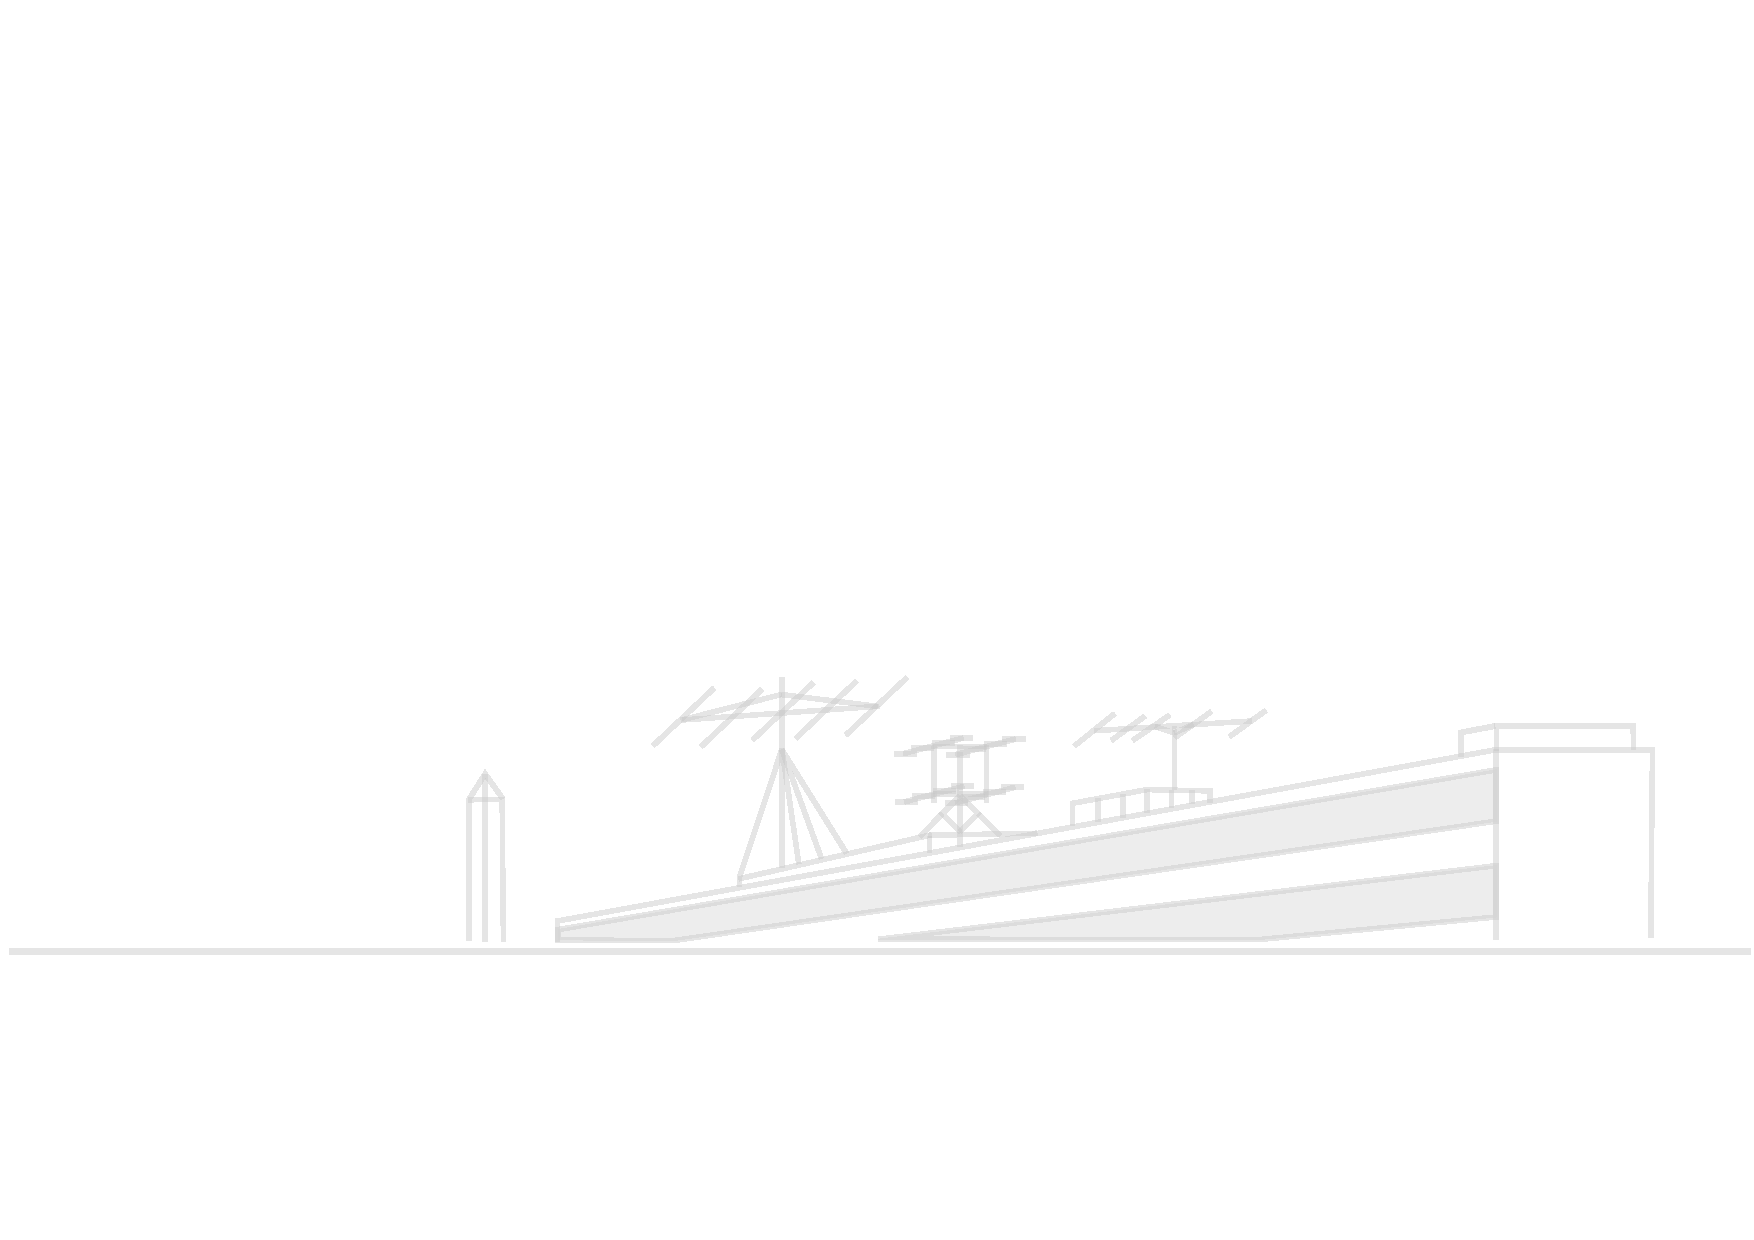
\includegraphics[width=17.8cm]{texdata/dk0tu_rooftop_background.pdf}
}

% Foliennummer einfügen
\setbeamertemplate{footline}[frame number]
%\setbeamertemplate{footline}{}

% Ändere das Zeichen vor jedem item
%\setbeamertemplate{itemize item}{\color{craneorange}$\blacktriangleright$}
%\setbeamertemplate{itemize subitem}{\color{craneorange}$\triangleright$}
%\setbeamertemplate{itemize subsubitem}{\color{craneorange}$\blacktriangleright$}

% Ändert die Blöcke 
\setbeamertemplate{blocks}[rounded][shadow=true]
% default | rounded [shadow=true|false]

%
% Eigene Kommandos
%

% Hack to get natbib and beamer working together. "The beamer user guide suggests
% that only the manual bibliography entry approach is supported"
% on some system it works out of the box, sometimes you need the hack :-(
% so check it --dl7bst
\ifdefined\newblock
    \relax
\else
    \newcommand{\newblock}{}
\fi

% \includedia command to generate png out of a dia file
% NEEDS installed dia and pdflatex option --shell-escape
\newcommand{\includedia}[1]{
    \immediate\write18{/usr/bin/dia #1.dia -e #1_diatmp.png -t png}
}

% RICHIG GROSSER FONT!
\newfont{\bigfont}{cmr10 at 144pt}
\newfont{\smallfont}{cmr10 at 8pt}

% Römische Ziffern
\makeatletter
\newcommand{\rmnum}[1]{\romannumeral #1}
\newcommand{\Rmnum}[1]{\expandafter\@slowromancap\romannumeral #1@}
\makeatother

% Schwarze Überschrift
%\setbeamercolor{frametitle}{fg=black}
%\setbeamercolor{title}{fg=black}

% Item- und Box-Farben
\definecolor{deepBlue}{HTML}{000066}
\setbeamercolor{itemize item}{fg=deepBlue}
\setbeamercolor{itemize subitem}{fg=deepBlue}
\setbeamercolor{description item}{fg=deepBlue}
\setbeamercolor{block title}{fg=deepBlue!100, bg=blue!15}
\setbeamercolor{block body}{fg=black, bg=blue!5}
\setbeamercolor{block title alerted}{fg=deepBlue, bg=red!75}
\setbeamercolor{block body alerted}{fg=black, bg=red!15}
\setbeamercolor*{block title example}{fg=blue!50, bg=blue!10}
\setbeamercolor*{block body example}{fg= blue, bg=blue!5}

%\setbeamercolor{section in head/foot}{parent=palette primary}
%\setbeamercolor{subsection in head/foot}{parent=palette secondary}
%\setbeamercolor{sidebar}{fg=darkblue,bg=yellow!90!orange}
%\setbeamercolor{title in sidebar}{fg=darkblue}
%\setbeamercolor{author in sidebar}{fg=darkblue}
%\setbeamercolor{section in sidebar}{fg=darkblue!10!black}
%\setbeamercolor{subsection in sidebar}{fg=darkblue!50!black}

% Titlepage Infos
\title{AFu-Kurs nach DJ4UF}
\author[DKØTU]{DKØTU\\ \footnotesize{Amateurfunkgruppe der TU Berlin}}
\institute[DKØTU]{\url{http://www.dk0tu.de} }

% PDF-Eigenschaften
\subject{DK0TU-Amateurfunkkurs nach DJ4UF}
\keywords{Amateurfunk Kurs HAM Radio Course CC-BY-NC-SA OpenSource TU Berlin DK0TU}

\subtitle{Technik A08: \\
           Das elektromagnetische Feld \\[2em]}
\date{Stand 02.06.2016}
 \begin{document}

\begin{frame}
    \titlepage
    \vfill
    \begin{center}
        \ccbyncsaeu\\
        {\tiny This work is licensed under the \em{Creative Commons Attribution-NonCommercial-ShareAlike 3.0 License}.}\\[0.5ex]
         \tiny Amateurfunkgruppe der Technische Universität Berlin (AfuTUB), DKØTU
         %\includegraphics[scale=0.5]{img/DK0TU_Logo.pdf}
    \end{center}
\end{frame}


\section*{Wiederholung}

\begin{frame}
    \frametitle{Wiederholung}
    \begin{center}
        % FIXME in erster Abbildung +/- und Pfeile nicht einzeichnen - siehe Praxis-Skript
		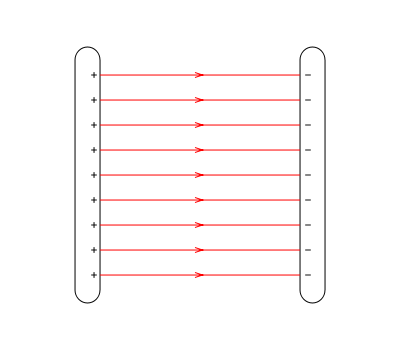
\includegraphics[width=\textwidth,height=.6\textheight,keepaspectratio]{e08/PlattenkondensatorFeld.png}\\
		\only<2>{\tiny Abb. 1: elektrisches Feld zwischen zwei leitenden Platten\\(CC-BY 3.0 \url{https://de.wikipedia.org/wiki/Benutzer:Wfstb})}
		\begin{itemize}
			\item Was für ein Feld ist dies?
			\item von wo nach wo gehen die Linien?
		\end{itemize}
	\end{center}
\end{frame}

\section*{Elektrisches Feld}

\begin{frame}
    \frametitle{Wie verlaufen die Feldlinien?}
    \begin{center}
        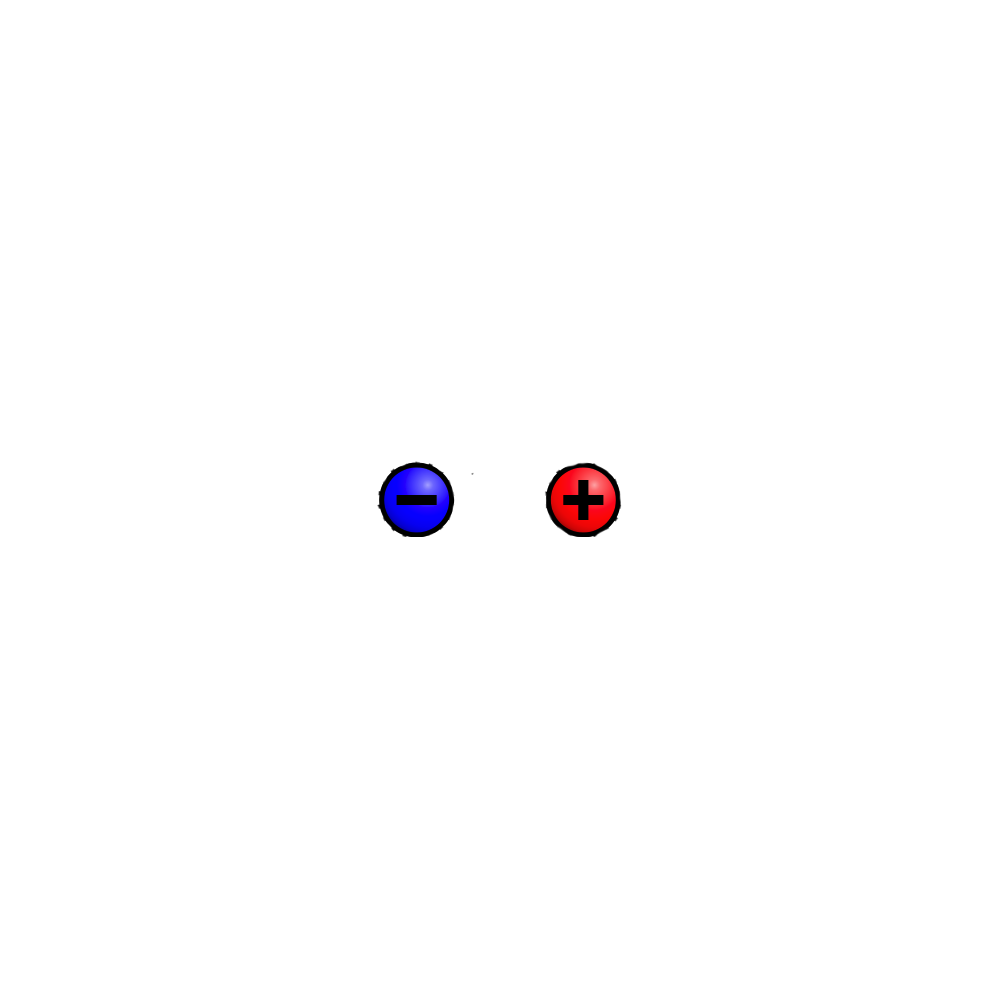
\includegraphics[width=0.8\textwidth,height=.8\textheight,keepaspectratio]{a08/VFPt_dipole_electric_ohne.png}
	{\tiny \hyperlink{refs}{\cite{wm}}}
    \end{center}
\end{frame}

\begin{frame}
    \frametitle{So verlaufen die Feldlinien}
    \begin{center}
        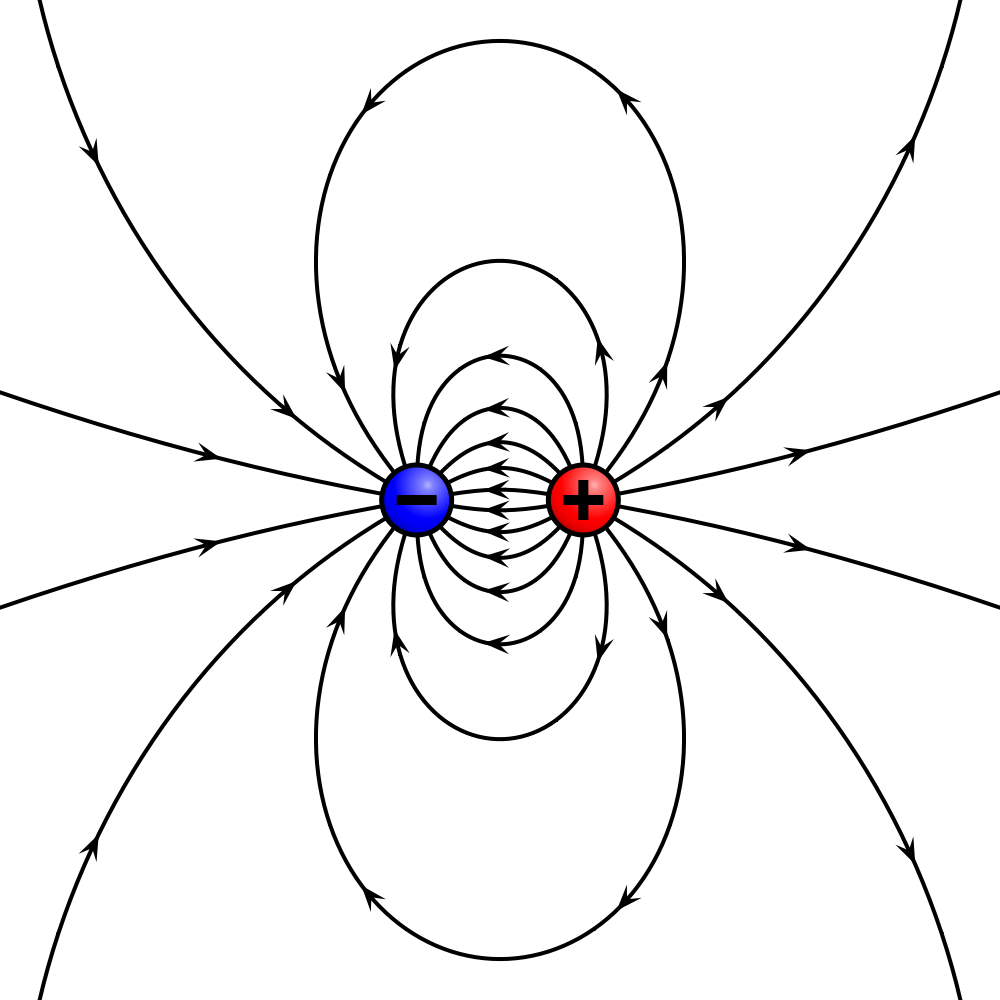
\includegraphics[width=0.8\textwidth,height=.8\textheight,keepaspectratio]{a08/VFPt_dipole_electric_mit.png}
	{\tiny \hyperlink{refs}{\cite{wm}}}
    \end{center}
\end{frame}

\begin{frame}
    \frametitle{Elektrisches Feld}
    \begin{block}{Elektrisches Feld}
    \begin{center}
        \huge $E = \cfrac{U}{d}$
    \end{center}
    \end{block}
\end{frame}

\begin{frame}
  \frametitle{Elektrisches Feld}
  \begin{exampleblock}{TB512}
    \begin{center}
      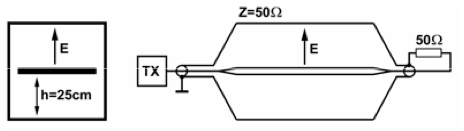
\includegraphics[width=1\textwidth,height=.4\textheight,keepaspectratio]{a08/TB512.png}
      {\tiny TB512 \hyperlink{refs}{\cite{bna}}}
    \end{center}
    \only<1>{Welche elektrische Feldstärke $E$ herrscht in der Mitte der dargestellten, symmetrisch aufgebauten Messzelle, wenn der angeschlossene Sender 1 Watt Ausgangsleistung liefert?}
    \only<2>{
    \begin{align*}
      \text{geg.: } P &= 1W \\
      E &= \frac{U}{d} \text{ mit } U = \sqrt{P \cdot R}
    \end{align*}}
    \only<3>{
    \begin{align*}
      E &= 28.3 \frac{V}{m}
    \end{align*}}
  \end{exampleblock}
\end{frame}

\begin{frame}
    \frametitle{Starkes Elektrisches Feld}
    \begin{center}
        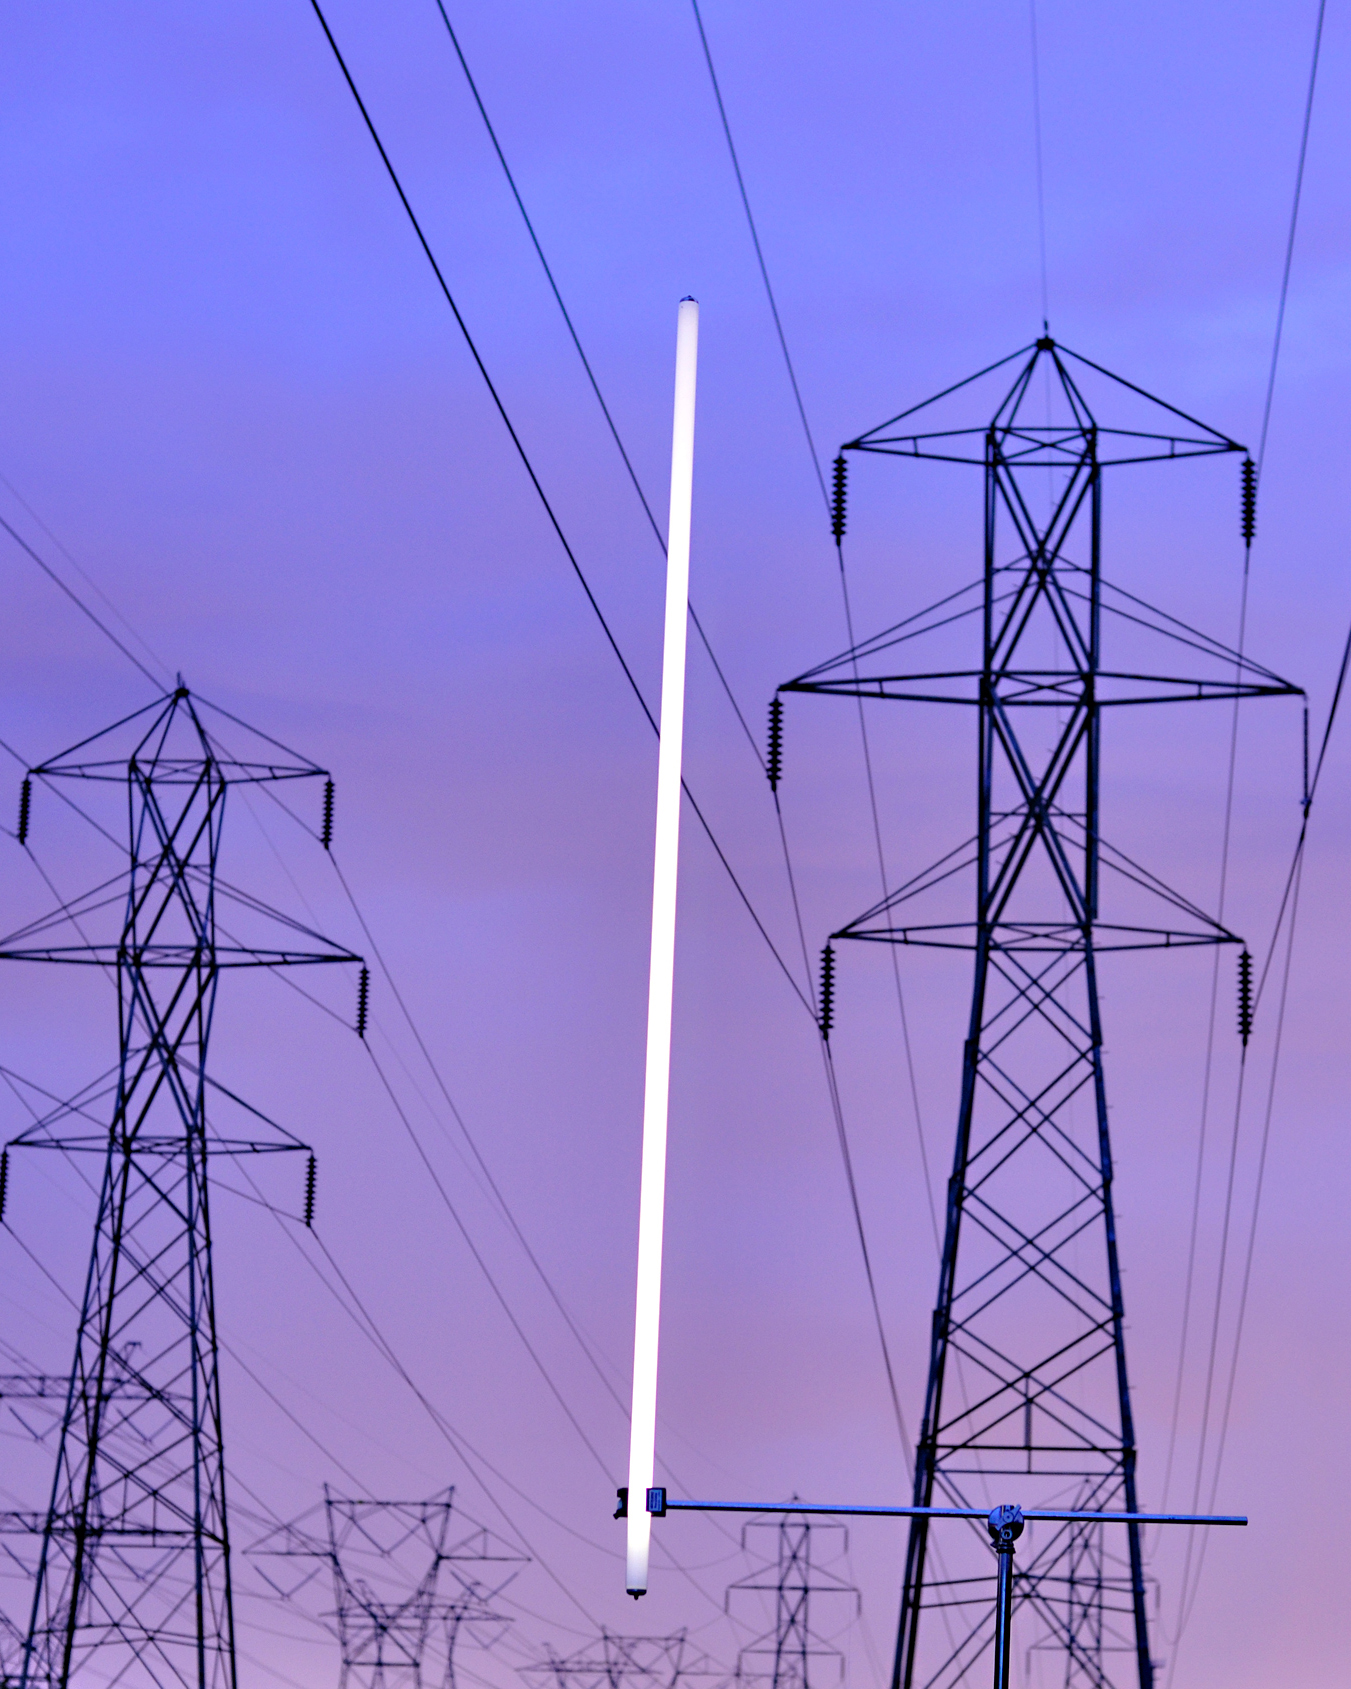
\includegraphics[width=0.6\textwidth,height=.85\textheight,keepaspectratio]{a08/Fluorescent_tube_under_electric_line.jpg}
	{\tiny \hyperlink{refs}{\cite{wm}}}
    \end{center}
\end{frame}

\section*{Magnetfeld}

\begin{frame}
    \frametitle{Magnetisches Feld}
    \begin{center}
		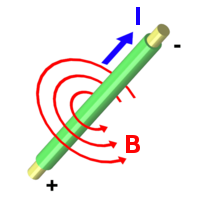
\includegraphics[width=0.6\textwidth,height=.6\textheight,keepaspectratio]{a08/RechteHand.png}\\
		{\tiny \hyperlink{refs}{\cite{wm}}} \\[1em]
		\begin{itemize}
			\item Rechte-Hand-Regel
			\item Magnetfeld um stromdurchflossenen Leiter
		\end{itemize}
	\end{center}
\end{frame}

\begin{frame}
    \frametitle{Stromdurchflossene Spule}
    \begin{center}
		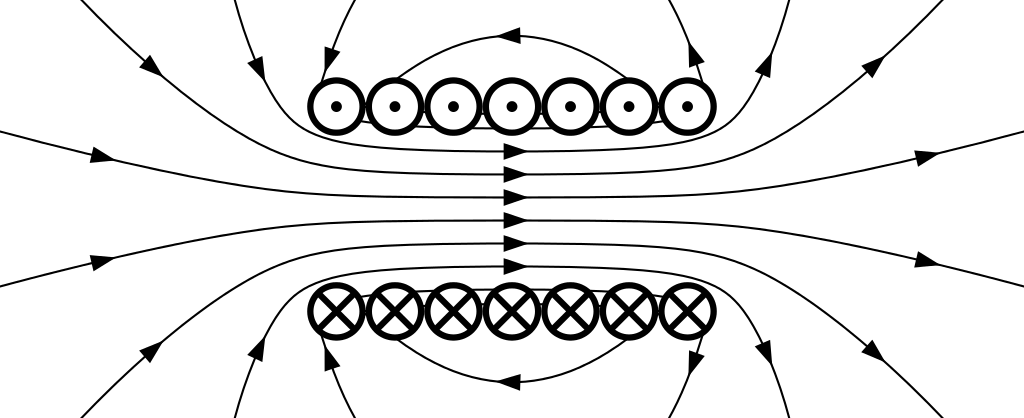
\includegraphics[width=0.7\textwidth,height=.6\textheight,keepaspectratio]{a08/H-Feld.png}\\
		{\tiny \hyperlink{refs}{\cite{wm}}} \\[1em]
		\begin{itemize}
		\item im Inneren ein homogenes magnetisches Feld
		\item Flussrichtung durch Rechte-Hand-Regel
		\end{itemize}
	\end{center}
\end{frame}

\begin{frame}
    \frametitle{3D-Darstellung}
    \begin{center}
		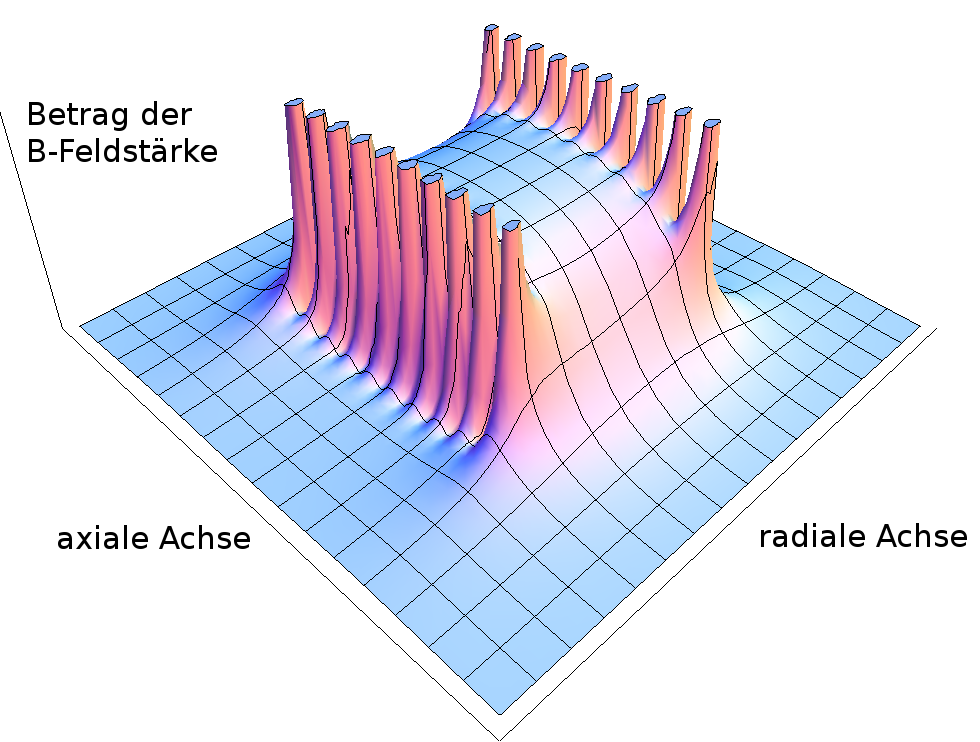
\includegraphics[width=0.7\textwidth,height=.6\textheight,keepaspectratio]{a08/3-D_HFeld.png}\\
		\tiny \hyperlink{refs}{\cite{wm}} \\[1em] \large
		\begin{itemize}
		\item Was ist das? Gibt es homogene Bereiche?
		\end{itemize}
	\end{center}
\end{frame}

\begin{frame}
    \frametitle{Formeln aus der Formelsammlung}
    \begin{block}{Formeln zur Spule}
      \begin{align*}
        \text{Feldstärke Leiter: } H &= \cfrac{\mathrm{I}}{\ell_m} \\[1em]
    	\text{Feldstärke Spule: } H &= \cfrac{\mathrm{I} \cdot N}{\ell_m} \\[1em]
	\text{Flussdichte Spule: } B &= \mu_r \cdot \mu_0 \cdot H \\[1em]
    	\mu_0 &= 1.257 \cdot 10^{-6}[\frac{Vs}{Am}] \\[1em]
	\mu_r &\approx 1 \text{ bei Luft}
     \end{align*}
   \end{block}
\end{frame}

\begin{frame}
  \frametitle{Induktionsofen}
  \begin{columns}[c]
    \column[c]{.6\textwidth}
    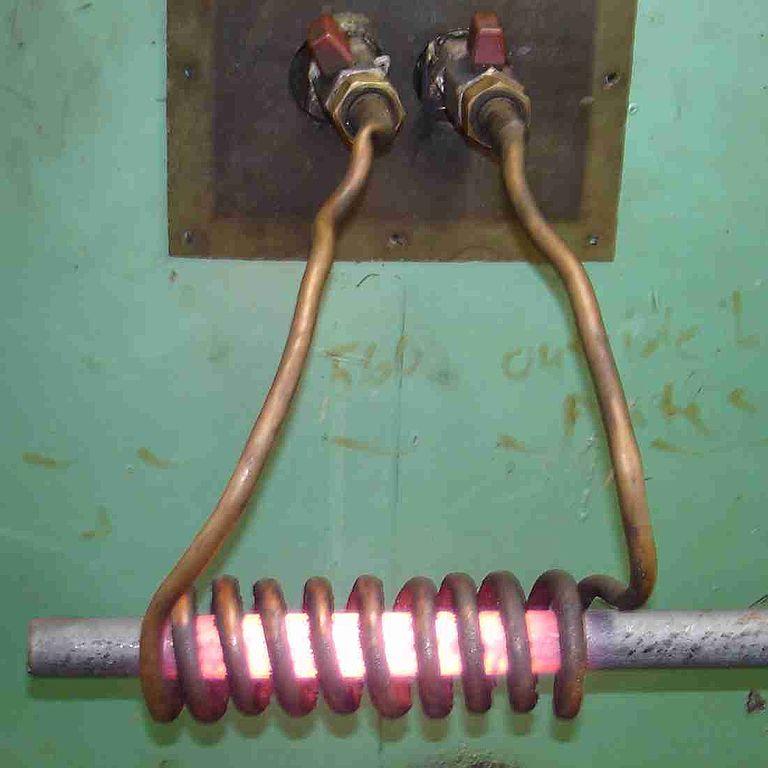
\includegraphics[width=\textwidth,height=.85\textheight,keepaspectratio]{a08/Induction_heating_of_bar_crop.jpg}\\
    {\tiny \hyperlink{refs}{\cite{wm}}} \\[1em]
    \column[c]{.35\textwidth}
    \begin{itemize}
	    \item $B = \mu \cdot H$ %(Flussdiche = Feldkonstante $\cdot$ Feldstärke)
        \item 15kW bei 450 kHz
      \item Spule ist wassergekühlt
    \end{itemize}
  \end{columns}
\end{frame}

\begin{frame}
  \frametitle{Hysterese}
  \begin{columns}[c]
    \column[c]{.49\textwidth}
    \begin{center}
      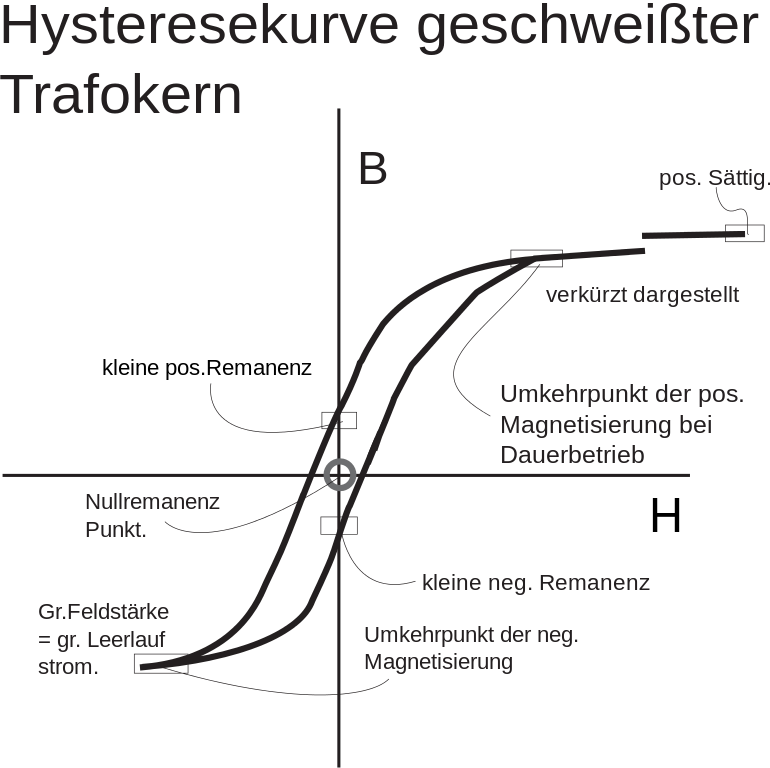
\includegraphics[width=1\textwidth,height=.8\textheight,keepaspectratio]{a08/Soft_hysteresis_welded.png}\\
      {\tiny \hyperlink{refs}{\cite{wm}}}
    \end{center}
    \column[c]{.49\textwidth}
    \begin{center}
      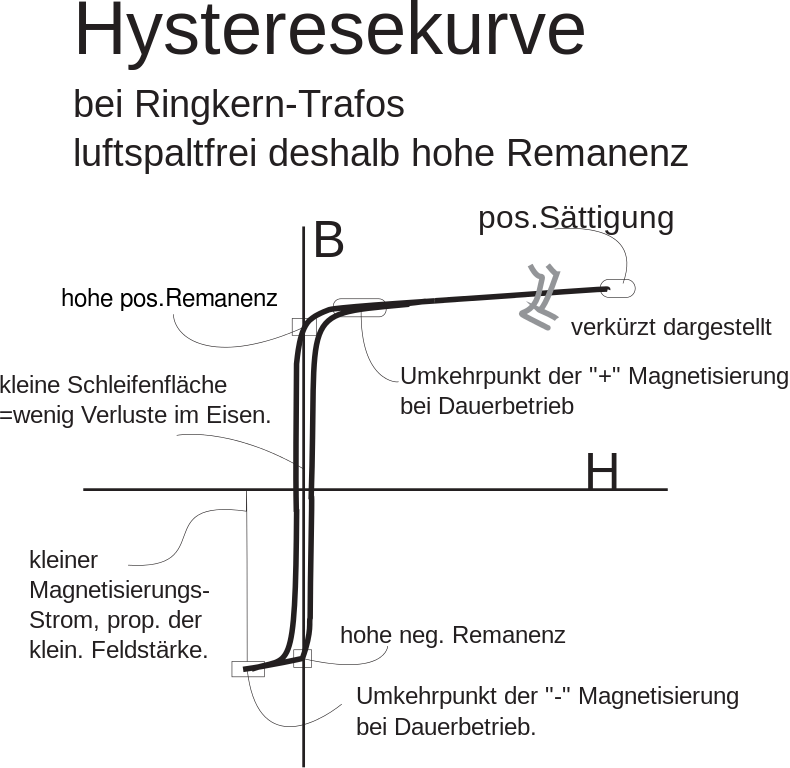
\includegraphics[width=1\textwidth,height=.8\textheight,keepaspectratio]{a08/Hard_hysteresis_de.png}\\
      {\tiny \hyperlink{refs}{\cite{wm}}}
    \end{center}
  \end{columns}
\end{frame}

\section*{Elektro"=magnetisches Feld}

\begin{frame}
  \frametitle{Verständnis Dipol}
  \begin{center}
    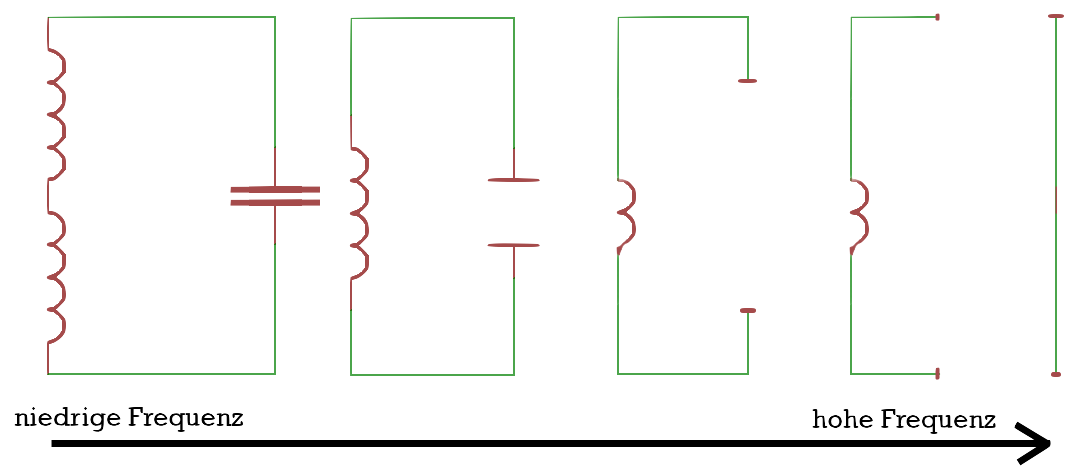
\includegraphics[width=1\textwidth,height=.85\textheight,keepaspectratio]{a08/dipol_entstehung.png}\\
  \end{center}
\end{frame}

\begin{frame}
  \frametitle{Das elektromagnetische Feld}
  \begin{center}
    %\animategraphics[loop,width=\textwidth,height=0.5\textheight,keepaspectratio,controls]{3}{e08/Dipolentstehung-}{0}{21}\\
    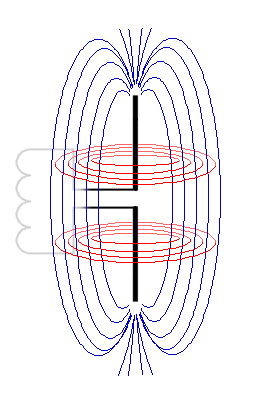
\includegraphics[width=1\textwidth,height=.5\textheight,keepaspectratio]{e08/Dipolentstehung-11.png}\\
    {\tiny elektromagnetisches Feld - siehe \url{../e08/Dipolentstehung.gif} \\
    {\tiny CC-BY-SA 3.0 \url{https://commons.wikimedia.org/wiki/File:Dipolentstehung.gif}}}
  \end{center}
  \begin{itemize}
    \item elektromagnetisches Feld bildet sich durch ein sich änderndes elektrisches und ein sich änderndes magnetisches Feld
    \item zieht man die Kondensatorplatten auseinander und streckt die Spule, erhält man eine Dipolantenne 
  \end{itemize}
\end{frame}

\section*{Fernfeld}

\begin{frame}
  \frametitle{Polarisation}
  \begin{center}
    \begin{minipage}{0.45\textwidth}
      %\animategraphics[loop,width=\textwidth,height=.6\textheight,keepaspectratio,controls]{8}{e08/Dipole_xmting_antenna_animation_4_408x318x150ms-}{0}{7}
        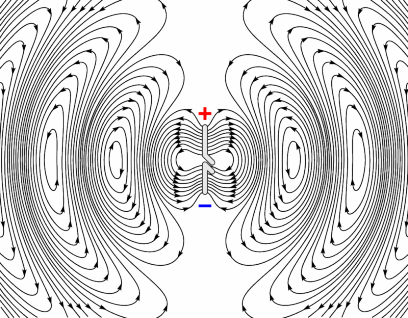
\includegraphics[width=1\textwidth,height=.6\textheight,keepaspectratio]{e08/Dipole_xmting_antenna_animation_4_408x318x150ms-2.png}\\
      {\tiny elektromagnetisches Feld einer Antenne \\
             siehe \url{../e08/Dipole_xmting_antenna_animation_4_408x318x150ms.gif}}
      %{\tiny (CC0) \url{https://de.wikipedia.org/wiki/Antennentechnik/media/File:Dipole_xmting_antenna_animation_4_408x318x150ms.gif}}}
    \end{minipage}
    \begin{minipage}{0.45\textwidth}
      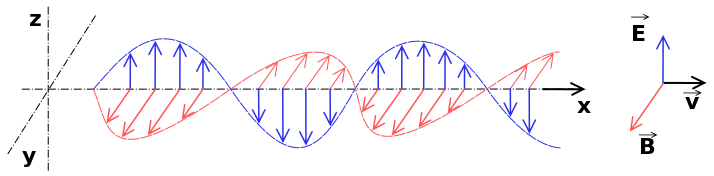
\includegraphics[width=\textwidth,height=.8\textheight,keepaspectratio]{e08/Onde_electromagnetique.png}\\
      {\tiny Polarisation einer Antenne}
      %{\tiny CC-BY-SA 3.0 \url{https://de.wikipedia.org/wiki/Antennentechnik/media/File:Onde_electromagnetique.svg}}}
      \begin{itemize}
	\item E-Feld bestimmt die Richtung der Polarisation
	\item magnetisches Feld ist um $90^\circ$ gedreht
	\item Im Amateurfunk horizontal oder vertikal
      \end{itemize}
    \end{minipage}\\[1.5em]
  \end{center}
\end{frame}

\begin{frame}
    \frametitle{Poynting-Vektor (nicht prüfungsrelevant)}
    \begin{center}
		\huge $$S = E \times H$$ \\[1em]
		\large Der Poynting-Vektor $S[\frac{W}{m^2}]$ ist das Kreuzprodukt aus dem $E$ und $H$ Feld gibt die Energierichtung, so wie die Wirkleistung des Signals an dem berechneten Punkt.
	\end{center}
\end{frame}

\begin{frame}
    \frametitle{Poynting-Vektor (nicht prüfungsrelevant)}
    \begin{center}
		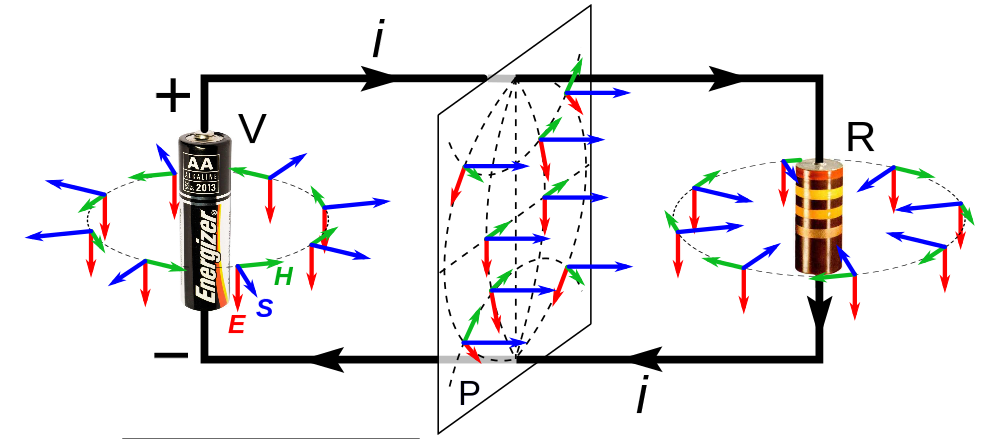
\includegraphics[width=1\textwidth]{a08/Poynting_vectors_of_DC_circuit.png}\\
		\tiny \hyperlink{refs}{\cite{wm}} \\[1em] \large
		Rot: E-Feld \\
		Grün: H-Feld
		Blau: Poynting
	\end{center}
\end{frame}

\begin{frame}
    \frametitle{Der Feldwellenwiderstand}
    \begin{block}{Feldwellenwiderstand}
      $E = Z_0 \cdot H$ \hspace{2cm} (analog zu $U = R \cdot I)$ \\[1em]
      Im Freiraum ist $Z_0$ eine Konstante: \\[1em]
      $Z_0 = \sqrt{\cfrac{\mu_0}{\varepsilon_0}} = 376,7 \Omega$ \\[1em]
  \end{block}
\end{frame}

\begin{frame}
    \frametitle{Die Ersatzfeldstärke}
    \begin{block}{Ersatzfeldstärke des E-Feldes}
        Im Fernfeld bei $> \frac{\lambda}{2\pi}$ (Herleitung nicht prüfungsrelevant)\\[1em]
    	$E = \cfrac{1}{r} \sqrt{\cfrac{Z_0}{4 \cdot \pi} \cdot P_s}$ \\[1em]
        Mit Freiraumdämpfung $Z_0 = 376,7 \Omega $\\[1em]
    	$\rightarrow E \approx \cfrac{\sqrt{30 \Omega \cdot P_s}}{r} $ \\[1em]
  \end{block}
\end{frame}

% Pause nicht notwendig
% \begin{frame}
%     \begin{center}
%         \Huge Pause
%     \end{center}
% \end{frame}

\begin{frame}
    \frametitle{Wellenlänge}
    \begin{center}
        \huge Wie lautet die Formel zum Umrechnen von Frequenz auf
        Wellenlänge?\footnote{zum ``Einbrennen'' ;-)}
    \end{center}
\end{frame}

\begin{frame}
    \frametitle{Wellenlänge}
    \begin{center}
        \huge $\lambda = \frac{300}{f}$ mit $f$ in $MHz$
    \end{center}
\end{frame}

\section*{Ionisations"=schichten}

\begin{frame}
    \frametitle{Raumwelle}
	\begin{center}
        % FIXME Grafiken aus dem Skript verwenden
        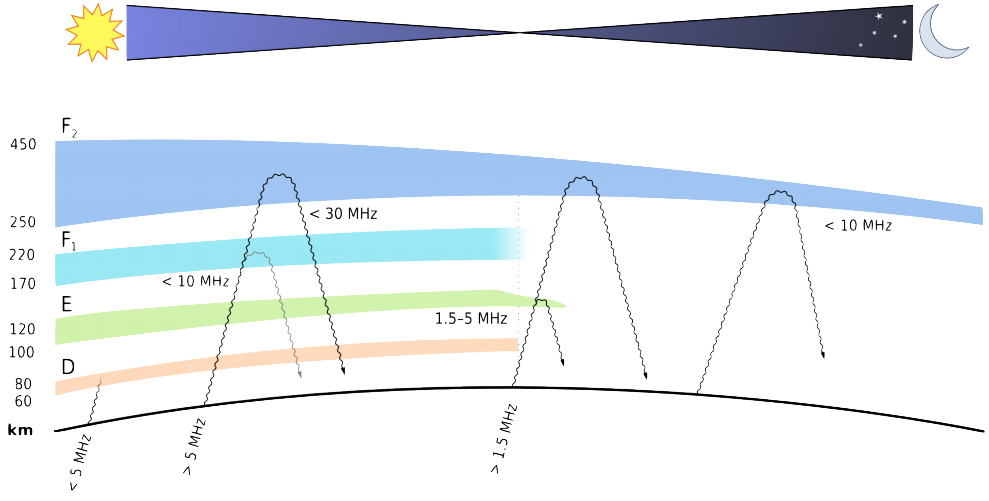
\includegraphics[width=.9\textwidth,height=.85\textheight,keepaspectratio]{a08/schichten_behelf_43.png}
        \footnote{\tiny Amateurfunkbehelf s.43 \url{http://ham.granjow.net/builds/Amateurfunkbehelf.pdf}}
    \end{center}
\end{frame}

\begin{frame}
    \frametitle{D-Schicht}
    \begin{itemize}
    			\item tagsüber und verschwindet nach Sonnenuntergang sehr schnell
				\item Dämpft Frequenzen unter $5MHz$ (160m und 80m unbenutzbar)
       		 	\item HF Frequenzen ab ca $20MHz$ sind bei einem Sonnenflecken-Minimum nicht verwendbar
       		 	\item bei hoher Sonnenaktivität
                      Mögel-Dellinger-Effekt\footnote{kurzzeitig ganzes KW-Band unbenutzbar}
    \end{itemize}
    \begin{center}
        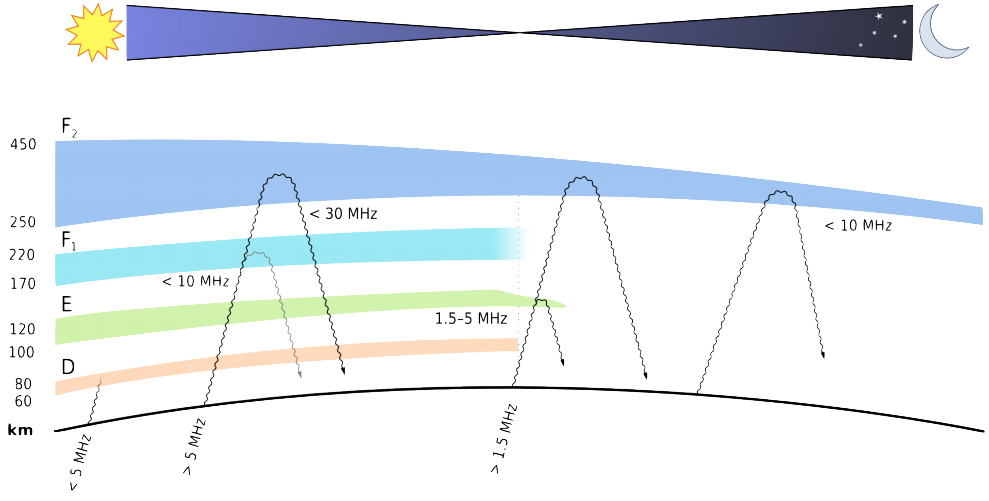
\includegraphics[width=.6\textwidth,height=.5\textheight,keepaspectratio]{a08/schichten_behelf_43.png}
        \footnote{\tiny Amateurfunkbehelf s.43 \url{http://ham.granjow.net/builds/Amateurfunkbehelf.pdf}}
    \end{center}
\end{frame}

\begin{frame}
    \frametitle{E-Schicht}
    \begin{itemize}
    			\item tagsüber
				\item reflektiert HF-Bänder 10m, 6m
       		 	\item reflektiert gelegentlich 2m (Sporadic-E) \footnote{\tiny \url{https://www.youtube.com/watch?v=xSWTkuSekhE}}
       		 	\item mit sehr starken Signalen zwischen 750 und 2200 km (Short-Skip)
    \end{itemize}
    \begin{center}
        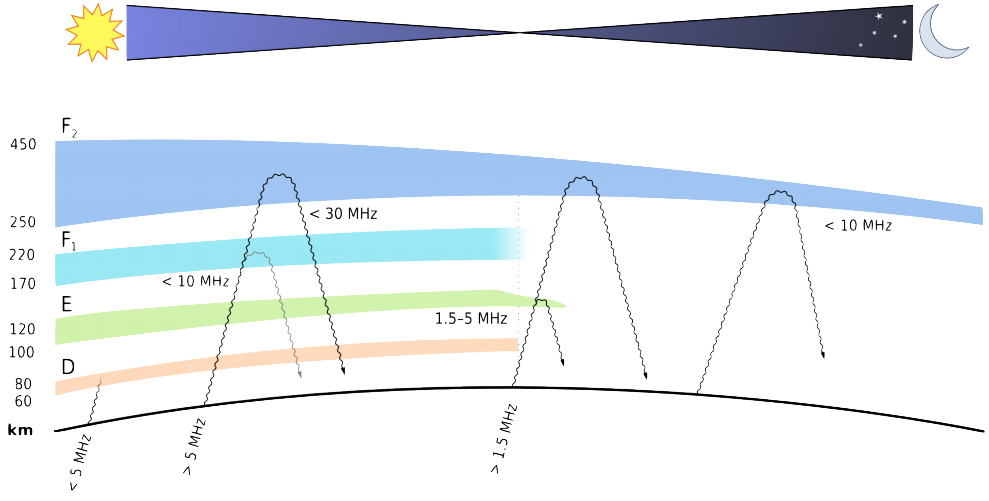
\includegraphics[width=.75\textwidth,height=.5\textheight,keepaspectratio]{a08/schichten_behelf_43.png}
        \footnote{\tiny Amateurfunkbehelf s.43 \url{http://ham.granjow.net/builds/Amateurfunkbehelf.pdf}}
    \end{center}
\end{frame}

\begin{frame}
    \frametitle{F-Schichten}
    \begin{itemize}
    			\item F1 und F2 Schicht
				\item F2 Schicht besteht auch Nachts (langsame Rekombination)
       		 	\item beständigste Schichten für KW
       		 	\item mit sehr starken Signalen zwischen 750 und 2200 km (Short-Skip)
    \end{itemize}
	\begin{center}
        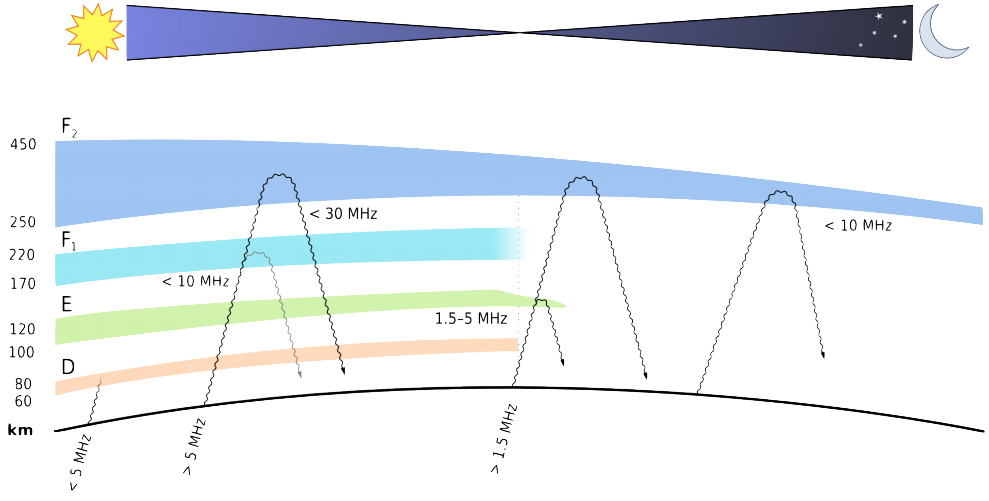
\includegraphics[width=.75\textwidth,height=.5\textheight,keepaspectratio]{a08/schichten_behelf_43.png}
        \footnote{\tiny Amateurfunkbehelf s.43 \url{http://ham.granjow.net/builds/Amateurfunkbehelf.pdf}}
    \end{center}
\end{frame}

\section*{Besondere Effekte}

\begin{frame}
    \frametitle{Solarer Flux}
    \begin{itemize}
    			\item Messwert der solaren Radiostrahlung bei $2800 MHz$
				\item Werte über 100 stehen für große Ionisation und somit gute Fernausbreitung von KW
    \end{itemize}
    \begin{center}
        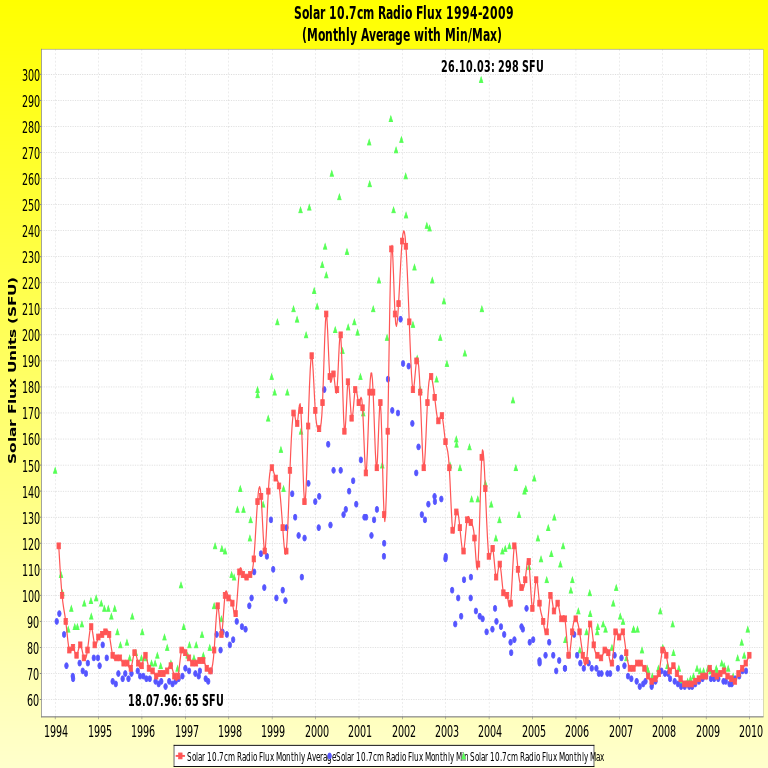
\includegraphics[width=.7\textwidth,height=.7\textheight,keepaspectratio]{a08/Solar_10_7_cm_Radio_Flux.png}
    \end{center}
\end{frame}

\begin{frame}
    \frametitle{MUF}
        \begin{center}
    \begin{itemize}
    			\item $MUF$: Größte noch nutzbare Frequenz für Reflektion
    			\item $MUF \approx \cfrac{f_{kritisch}}{sin{\alpha}} = \cfrac{f_{kritisch}}{cos{\phi}}$
				\item $\alpha$ ist der Abstrahlwinkel vom Boden
				\item $\phi$ ist der Auftreffwinkel auf die Schicht
				\item $f_{opt} = 0.85 \cdot MUF$
    \end{itemize}
        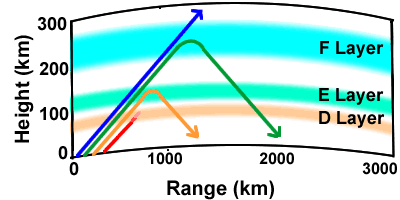
\includegraphics[width=.6\textwidth,height=.4\textheight,keepaspectratio]{a08/DifferentFrequencies-NPS.png}
    \end{center}
\end{frame}

\begin{frame}
  \begin{tabular}{l||p{.8\textwidth}}\hline
    \textbf{TI227} & \textbf{Berechnen Sie die höchste brauchbare Frequenz (MUF) und die optimale Frequenz ($f_{opt}$) für einen Abstrahlwinkel von $45^\circ$, wenn für den zu berechnenden Tag eine kritische Grenzfrequenz von $f_k = 3 MHz$ gemessen wurde.}\\ \hline\hline
    A & $MUF=2,1MHz$, $f_{opt} = 1,8MHz$ \\ \hline
    B \only<2>\checkmark & $MUF=4,2MHz$, $f_{opt} = 3,6MHz$ \\ \hline
    C & $MUF=2,1MHz$, $f_{opt} = 2,5MHz$ \\ \hline
    D & $MUF=4,2MHz$, $f_{opt} = 4,9MHz$ \\ \hline
  \end{tabular}
\end{frame}

\begin{frame}
    \frametitle{Fading, Backscatter}
        \begin{center}
    \begin{itemize}
    			\item Von Fading spricht man, wenn während eines Durchgangs aufgrund von unterschiedlich starker Ionisierung der Schichten das Signal mal stärker und mal schwächer zu empfangen ist
    			\item Backscatter bezeichnet die Rückstreuung von Wellen und kann bei Frequenzen weit über der MUF auftreten wenn die Ionosphäre inhomogen ist  			
    			\item \url{https://upload.wikimedia.org/wikipedia/commons/c/c6/Radaroperation.gif}
    			\item Wird bei Radaren genutzt
    \end{itemize}
    \end{center}
\end{frame}

\begin{frame}
    \frametitle{Mögel-Dellinger}
    \begin{center}
    \begin{itemize}
    			\item Entdeckt wurde der Effekt um das Jahr 1930 von Hans Mögel, 1935 hat ihn der John Howard Dellinger dem US-Standardisierungsamt (National Bureau of Standards) vorgestellt
    			\item Durch Sonneneruptionen, sogenannten Flares, werden kurzzeitig alle Frequenzen unterhalb von $300MHz$ stark gedämpft durch Ionisierung der D-Schicht
    			\item Im Bild ist blau Normal und rot nach dem Flare. \\[1em]
    \end{itemize}
        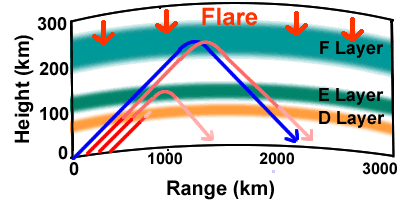
\includegraphics[width=.6\textwidth,height=.4\textheight,keepaspectratio]{a08/FlareNPS.png}
    \end{center}
\end{frame}

\begin{frame}
        \begin{center}
        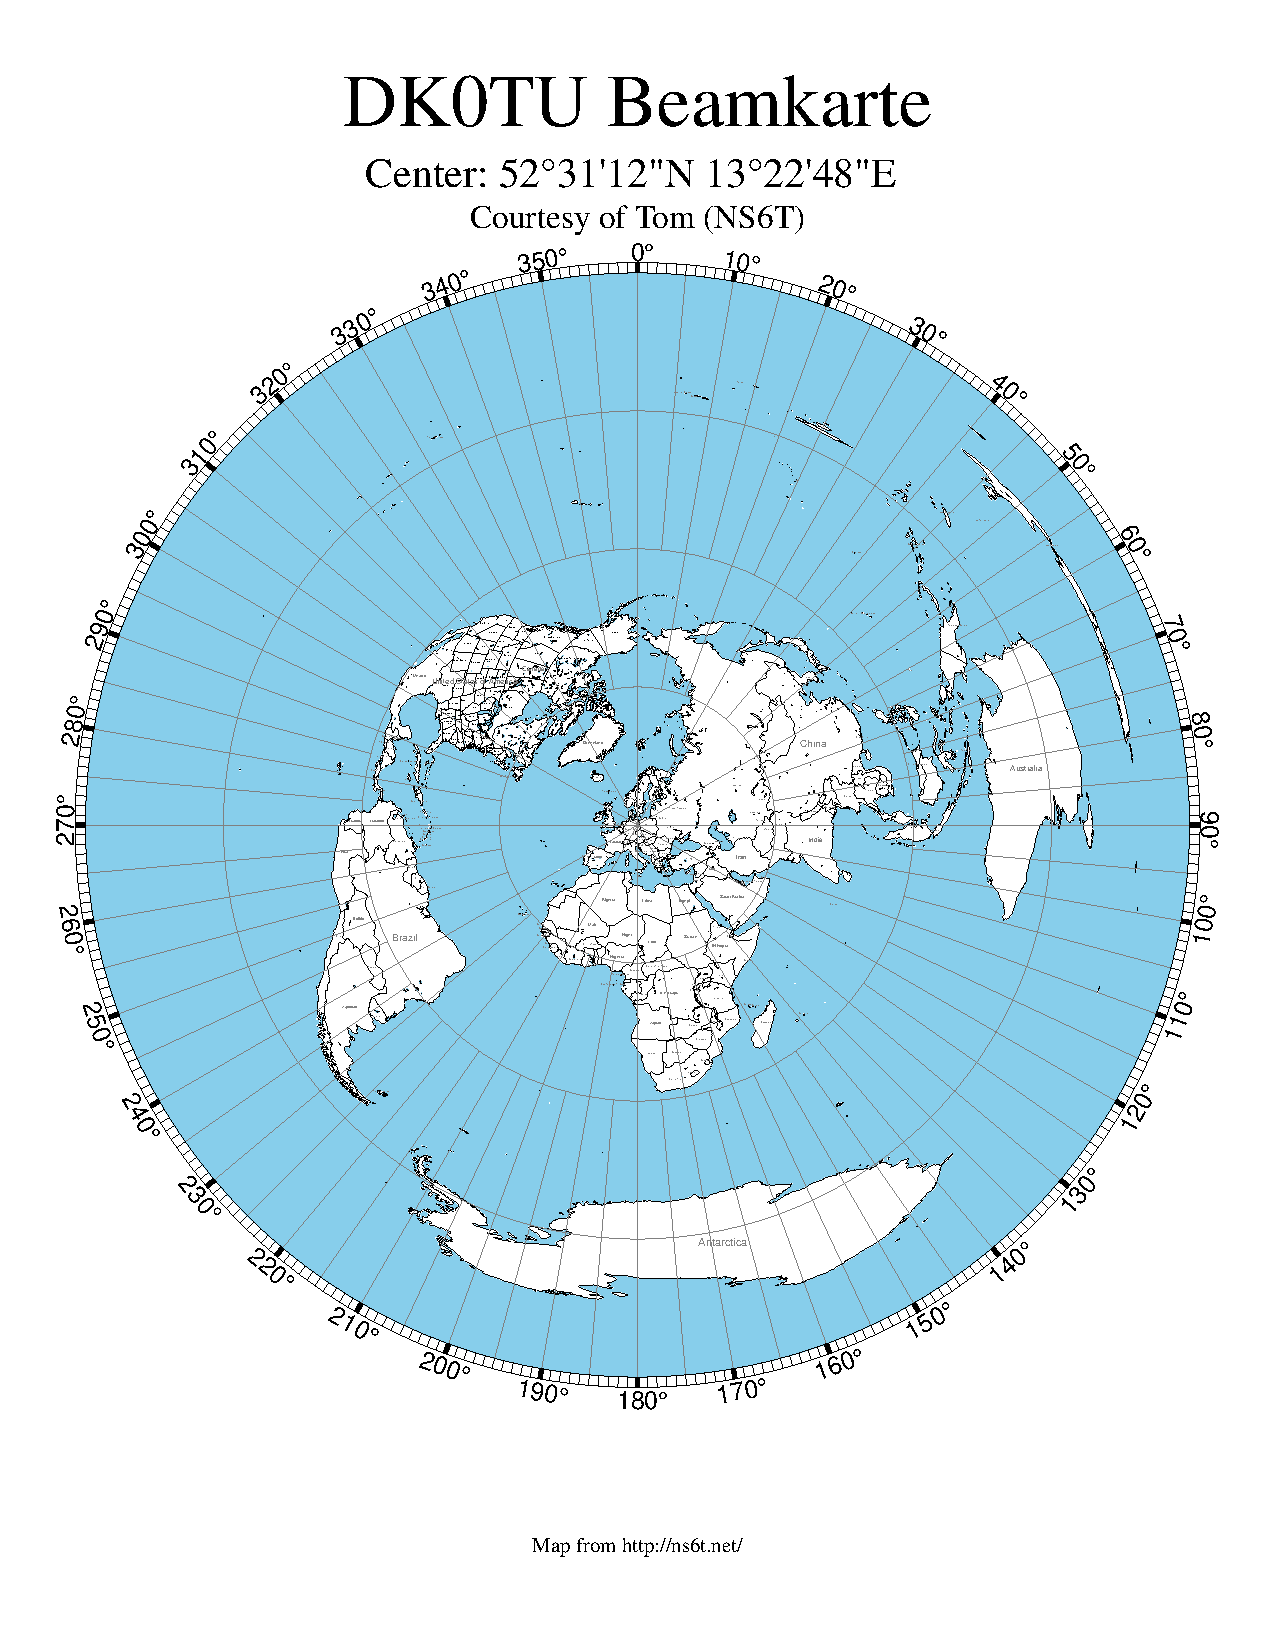
\includegraphics[height=\textheight,height=\textheight,keepaspectratio]{a08/AzimuthalMap.pdf}
    \end{center}
\end{frame}

\begin{frame}
    \frametitle{Reichweite der Bänder}
    \begin{center}
    \begin{itemize}
    			\item Welche Bänder tagsüber?
    			\item Welche Bänder nachts?
    			\item Womit geht mehr DX?
    			\item \url{http://www.dr1a.com/pages/de/dx-propagation.php}
    			\item Ausführlich auch in E-Technik E09
    \end{itemize}
    \end{center}
\end{frame}

\begin{frame}
  \begin{exampleblock}{Hausaufgabe}
    Prüfungskatalog Kapitel 1.9.1 Ionosphäre, TI101--TI115\\
    Prüfungskatalog Kapitel 1.9.2 Kurzwellenausbreitung, TI201--TI239\\
    Prüfungskatalog Kapitel 1.9.3 Wellenausbreitung oberhalb 30MHz, TI301--TI317
  \end{exampleblock}
\end{frame}

\renewcommand{\refname}{Referenzen}

\hypertarget{refs}{}
\textcolor{white}{} \\ %\vspace{} geht nicht
\Large Referenzen/Links
\footnotesize

\begin{thebibliography}{}
    \bibitem{darc}  DARC Online-Lehrgang Lektion A08:
                    \url{http://www.darc.de/referate/ajw/ausbildung/darc-online-lehrgang/technik-klasse-a/technik-a08/}
    \bibitem{wm} 	Wikimedia:
                    \url{https://commons.wikimedia.org/wiki/File:VFPt_dipole_electric.svg}
                    \url{https://de.wikipedia.org/wiki/Datei:Fluorescent_tube_under_electric_line.jpg}
                    \url{https://commons.wikimedia.org/wiki/File:RechteHand.png}
                    \url{https://commons.wikimedia.org/wiki/File:Solenoid.png}
                    \url{https://commons.wikimedia.org/wiki/File:VFPt_Solenoid_correct2.svg}
                    \url{https://de.wikipedia.org/wiki/Datei:Induction_heating_of_bar_crop.jpg}
                    \url{https://de.wikipedia.org/wiki/Datei:Soft_hysteresis_welded.svg}
                    \url{https://commons.wikimedia.org/wiki/File:Onde_electromagnetique.svg}
                    \url{https://commons.wikimedia.org/wiki/File:Poynting_vectors_of_DC_circuit.svg}
                    \url{https://commons.wikimedia.org/wiki/File:FlareNPS.gif}
                    \url{}
                    \url{}
                    \url{}
                    \url{}
    \bibitem{beam}  Beamkarten Generator von NS6T:
                    \url{http://ns6t.net/azimuth/azimuth.html}
    \bibitem{wp}    Wikipedia - Die freie Enzyklopädie:
                    \url{https://de.wikipedia.org/wiki/Elektrisches_Feld}
	\bibitem{bna}   Fragenkatalog Bundesnetzagentur Technik Klasse A:                   
                    \url{https://www.bundesnetzagentur.de/SharedDocs/Downloads/DE/Sachgebiete/Telekommunikation/Unternehmen_Institutionen/Frequenzen/Amateurfunk/Fragenkatalog/TechnikFragenkatalogKlasseAf252rId9014pdf.pdf?__blob=publicationFile&v=3}
\end{thebibliography} 

% Hier könnte noch eine Kontaktfolie stehen

\end{document}

